\subsection{Administrator Stakeholders}
\label{sec:administrative_stakeholders}

With the underlying data structures explained, it is now clear how
{\em Via} builds special subgraphs by filtering early, when the
student level information is still available. The filtering occurs as
matrix $M$ is constructed. Similarly, the discount function is used to
control how closely together we wish enrollments to have occurred in
time. The following application takes advantage of the adjacency
matrix itself, not explicitly creating a graph.

Our model provides an intuitive medium for understanding
department-wide dynamics across varying student
demographics. Administrators in charge of course resource allocation
may be interested in the enrollment patterns of students as they move
through a department's course offerings. We provide two use cases to
illustrate how \textit{Via} can be leveraged to derive insights into
the structure of courses within departments.

First, we study which classes tend to guide a student into a certain
department. We report the top 10 classes within a department that,
once taken by a student, have the highest average number of subsequent
enrollments within the same department. In
Figure~\ref{fig:persistence} we show the student persistence within a

\begin{figure*}[h!]
    \centering
    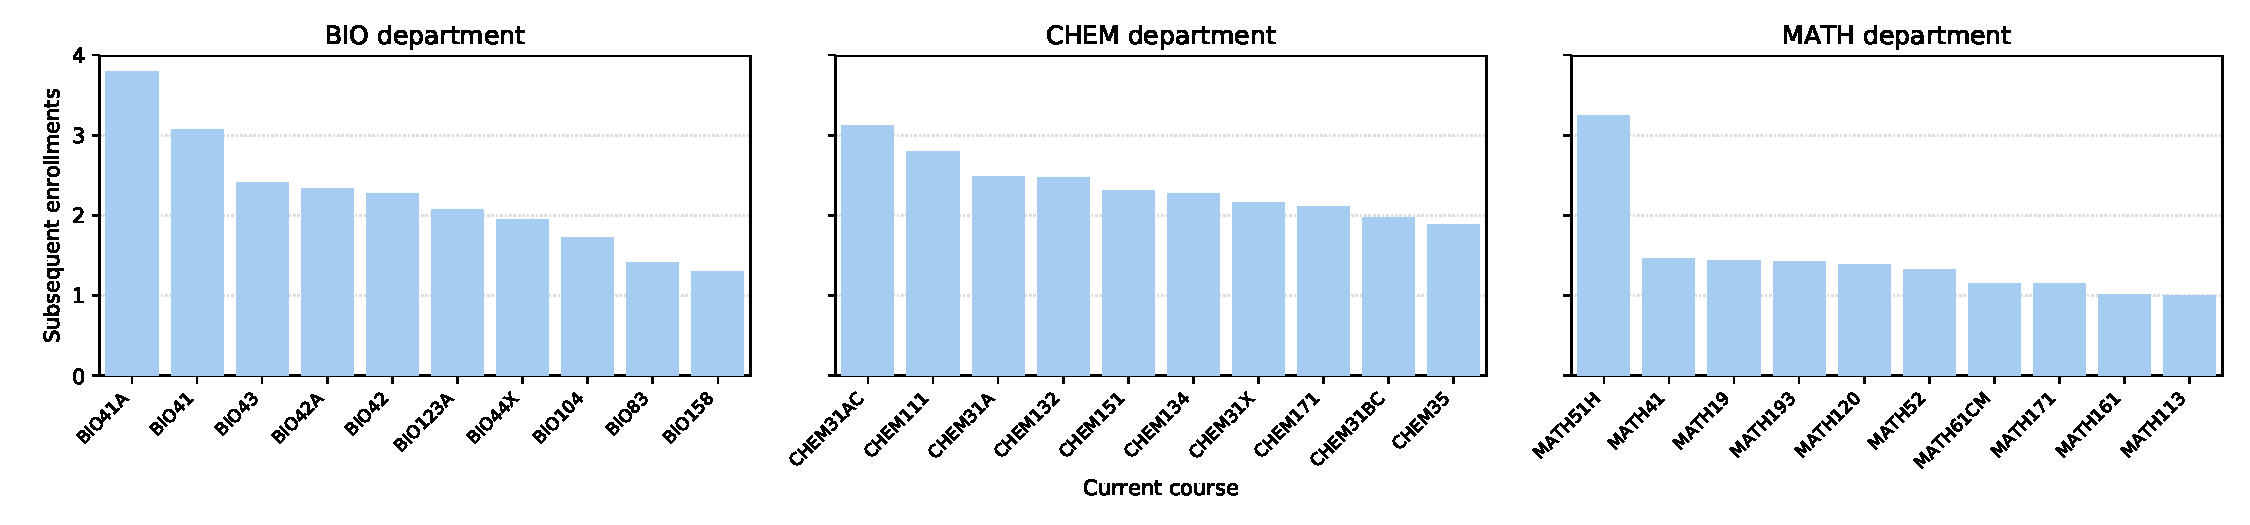
\includegraphics[width=18cm]{Figs/final-persistence.pdf}
    \caption{Student persistence metrics in Biology, Chemistry and
      Mathematics. The support courses for the biology and chemistry
      departments' introductory courses, \textsc{bio41a} and \textsc{chem31ac},
      respectively, lead to higher subsequent enrollment rates within
      the respective departments.}
    \label{fig:persistence}
\end{figure*}

department using a raw count projection model with discrete discount
function $d$ that captured all non-co-enrollment relationships between
courses from 2014-2018.  This ``persistence within a department''
metric can be computed for a given class $i$ in a department $x$ by
finding the out-degree of the class node and then dividing by the
total number of students who enrolled in class $i$. This method is
equivalent to finding the expected number of courses taken within
department $x$ after enrollment in class $i$. Observe that this is
robust to a course's discontinuation across academic years due to the
conditions under which the ratio is calculated. Here we measure the
average number of courses taken within a department after having
enrolled in a given course. Within the Biology and Chemistry
departments, we recover the insight that the 1-unit companion courses
to the introductory courses (\textsc{bio41a} and \textsc{chem31ac} for
Biology and Chemistry, respectively) increased student
persistence. Intuitively, this observation indicates that enrollment
in these courses led to an overall increase in the number of courses
taken within the department, on average. We contrast this with the
Math department. Students who enrolled in the most courses offered
within the Math department were those who enrolled in the first course
of the honors multivariable mathematics sequence,
\textsc{math51h}. This observation can be explained by the fact that
the classes in the primary introductory course sequence in the Math
department (\textsc{math51}, \textsc{math52}, \textsc{math53}) often
serve as prerequisite courses for classes in other departments in
engineering and social sciences. Enrolling in the honors-level
mathematics sequence perhaps indicates a given student's higher
intrinsic inclination to the subject matter.
